%\begin{figure}[htbp]

  
%\begin{subfigure}{0.49\textwidth}
%    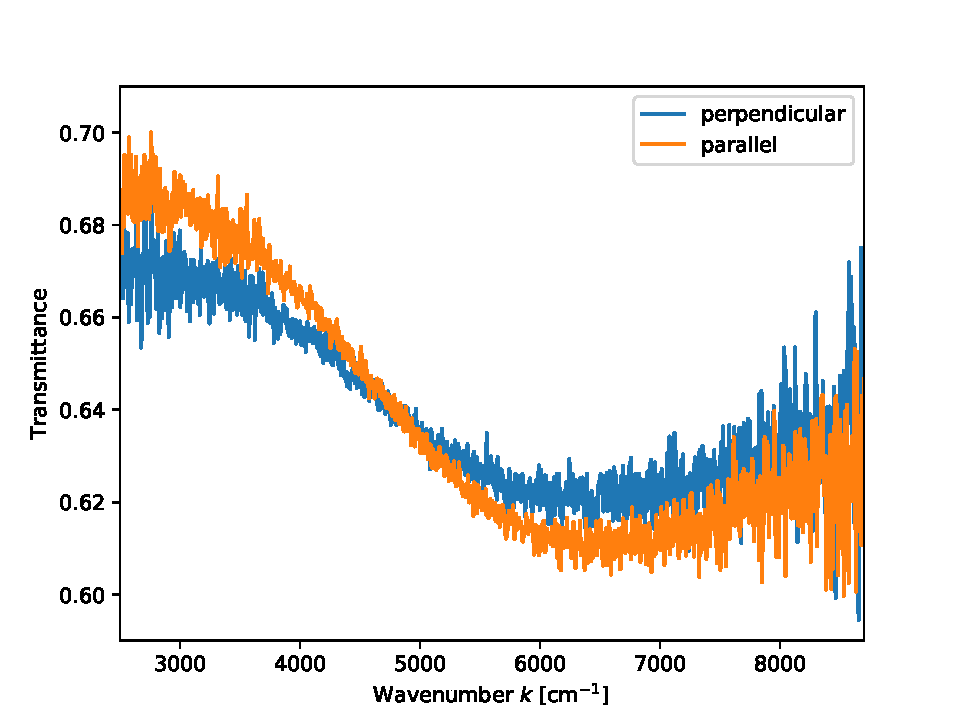
\includegraphics[width=\textwidth]{fullring.pdf}
%    \caption{fullrings  }
%    \label{fig:ftir_fr}
%\end{subfigure}
%\hfill
%\begin{subfigure}{0.49\textwidth}
%    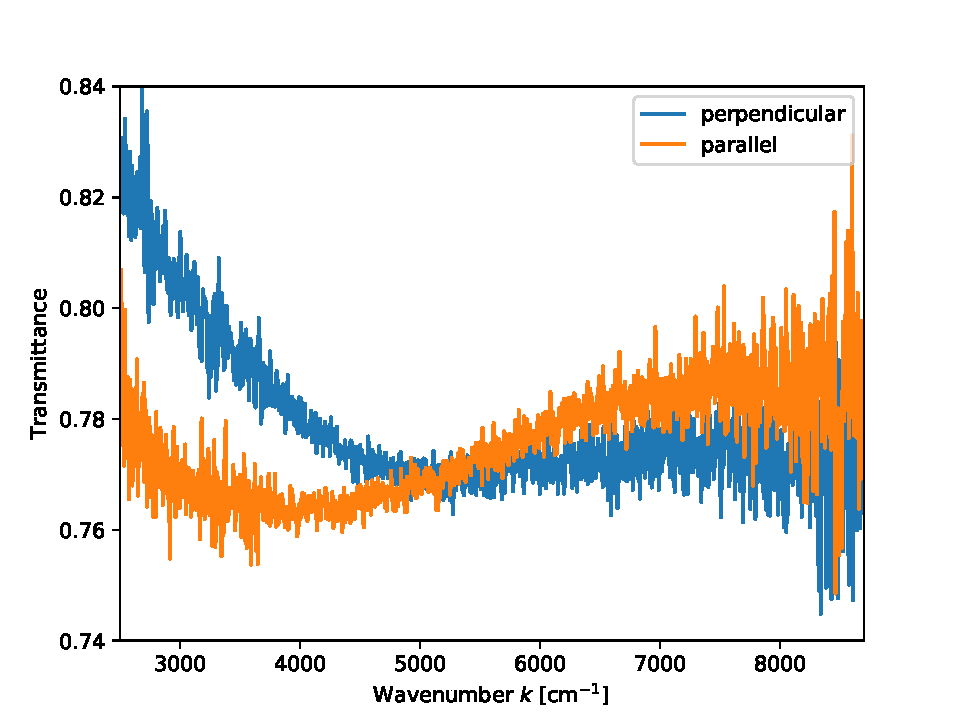
\includegraphics[width=\textwidth]{splitring.pdf}
%    \caption{splitrings}
%    \label{fig:ftir_sr}
%\end{subfigure}
%\caption{Transmittance spectra of fullrings (1) and splitrings (2) with a gap of $90^{\circ}$ between two different polarisations. }
%\label{fig:ftir}
  %\end{figure}

  \begin{figure}
   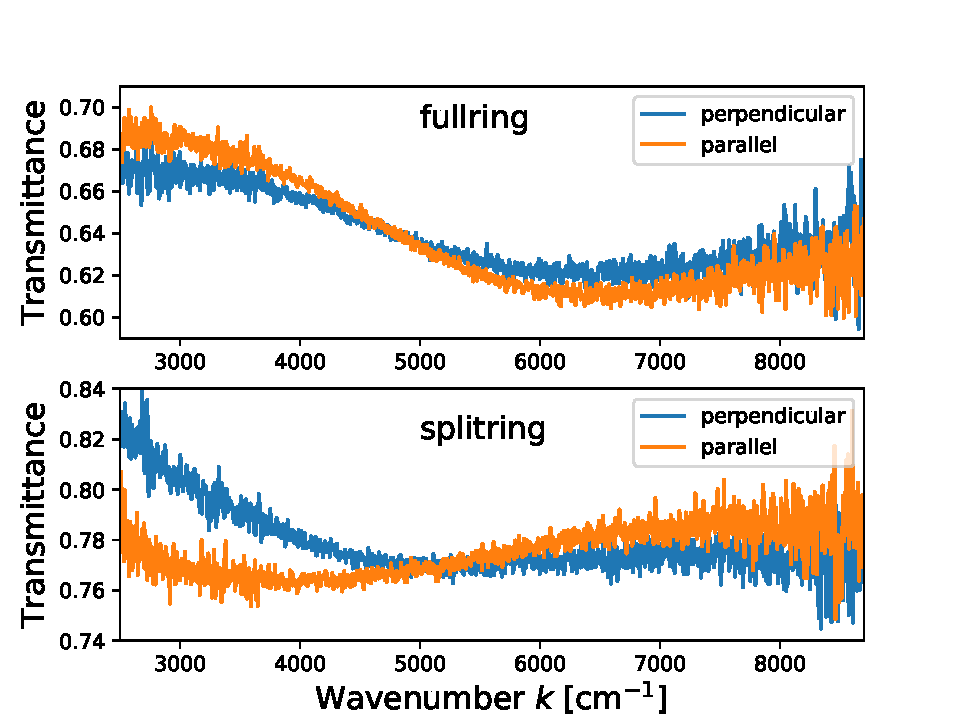
\includegraphics[scale=1.85]{FTIR.pdf}
  \caption{Transmittance spectra of fullrings  and splitrings  with a gap of $90^{\circ}$ between two different polarisations. }
  \label{fig:ftir}
  \end{figure}
  
\begin{itemize}
 \item{Fourier-transform infrared spectroscopy (FTIR) is a technique to measure the transmission infrared spectra of a  solids, liquid or gas.} 
\item{There are no different plasmonen modes visible in the transmission spectra.}
\item{The difference for the SRRs between the two polarisations is too small in comparison to the theory. }
\item{The polarisation has an effect for the fullrings, which should't be the case. }
  \end{itemize}
